\section{Multimodal fusion\label{multimodal:fusion}}

Here, we will illustrate here two types of multimodal integration:
\begin{enumerate}
 \item ``Fusion'' of the EEG and MEG data (Henson et al, 2009b),
 \item Use of the fMRI data as spatial priors on the MEG/EEG data (Henson et al, in press).
\end{enumerate}

\subsection{EEG and MEG fusion \label{multimodal:fusion:eegmeg:fusion}}

Make a new directory called ``Fused', and change into it.

\subsubsection{Merging the EEG and MEG datafiles \label{multimodal:fusion:eegmeg:merge}}

The first step is to combine the MEG and EEG data into a single SPM file. We will use the (weighted) averaged files for each modality.

Press ``Fuse'' from the ``Others'' pulldown menu, and select the MEG \texttt{wmcdbespm8\_\-SPM\_\-CTF\_\-MEG\_\-example\_\-faces1\_\-3D.mat} and \texttt{wmaceMdspm8\_faces\_run1.mat}. This will create a new file called \texttt{uwmcdbespm8\_\-SPM\_\-CTF\_\-MEG\_\-example\_\-faces1\_\-3D.mat}. Note that the two files need to have the same number of trials, conditions, samples, etc. Display the new file, and you will see the EEG and MEG data within their respective tabs.

We have to do one extra bit of ``preparation'' for the EEG data. Because in general, one might want to merge more than one EEG file, integrating all their locations could be tricky. So the simple answer is to clear all locations and force the user to re-specify them. So (as in previous EEG section), select \textsc{Prepare} from the ``Other'' menu and select \texttt{wmaceMdspm8\_faces\_run1.mat}. Then in the SPM Interactive window, on the ``Sensors'' submenu, choose ``Load EEG sensors''/``Convert locations file'', and select the \texttt{electrode\_locations\_and\_headshape.sfp} file (in the original EEG directory). Then from the ``2D projection'' submenu select ``Project 3D (EEG)''. A 2D channel layout will appear in the Graphics window. Select ``Apply'' from ``2D Projection'' and ``Save'' from ``File'' submenu.

\subsubsection{3D fused ``imaging'' reconstruction \label{multimodal:fusion:eegmeg:3D}}

Now we can demonstrate simultaneous reconstruction of the MEG and EEG data, as described in Henson et al (2009b). This essentially involves scaling each type of data and gain matrix, concatenating them, and inverting using the normal methods, but with separate sensor error covariance terms for each modality.
\begin{itemize}
\item Press the ``3D source reconstruction'' button, and load the \texttt{uwmcdbespm8\_\-SPM\_\-CTF\_\-MEG\_\-example\_\-faces1\_\-3D.mat} file. Type a label (eg ``N/M170'').

\item Press the ``MRI'' button, select the \texttt{smri.img} file within the \texttt{sMRI} sub-directory, and select ``normal'' for the cortical mesh. Because this MRI was normalised previous, this step should not take long, finishing with display of the cortex (blue), inner skull (red), outer skull (orange) and scalp (pink) meshes.

\item Press the ``Co-register'' button. Press ``type'' and for ``nas'', enter [0 91 -28] for ``lpa'' press ``type'' and enter [-72 4 -59] for ``rpa'' press ``type'' and enter [71 -6 -62]. Finally, answer ``yes'' to ``Use headshape points?''. Then select either ``EEG'' or ``MEG'' to display corresponding
data registration. Note that the MEG data will have been coregistered to the EEG data in the headspace. If you want to display the other modality afterwards, just press the ``display'' button below the ``Co-register'' button.

\item Press ``Forward Model'', and select ``EEG BEM'' for the EEG and ``Single Shell'' for the MEG. Then select either ``EEG'' or ``MEG'' to display corresponding forward model. (If you want to display the other modality afterwards, just press the ``display'' button below the ``Forward Model'' button). In the Graphics window the meshes will be displayed with the sensors marked with green asterisks.

\item Press ``save'' to save progress.

\item Press ``Invert'', select ``Imaging'', press ''yes'' for ''all conditions or trials'', ``Standard'' to use the default inversion settings (MSP), and then to the prompt ``Multiple modalities'', press ``fuse''.

%In order to compare with fMRI priors below, should really: select ``no'' to the question about ''all conditions or trials'', press ''yes'' to invert the Difference (between faces and scrambled) but ''no'' to invert the Mean (of faces and scrambled versus baselin). Then press ``Standard'' to use the default inversion settings (MSP), and to the prompt ''Multiple modalities'', press ''fuse''. but the fused and MEG results are not as convincing, for some reason...

At the first stage of the inversion lead fields will be computed for all the mesh vertices and saved in the file \texttt{SPMgainmatrix\_uwmcdbespm8\_SPM\_CTF\_MEG\_example\_faces1\_3D\_1.mat}. 
This will take some time.
Then the actual MSP algorithm will run and the summary of the solution will be displayed in the Graphics window.

\item Press ``save'' to save the results. You can now explore the results via the 3D reconstruction window. If you type 170 into the box in the bottom right (corresponding to the time in ms) and press ``mip'', you should see an output similar to Figure~\ref{multimodal:fusion:fig:1}.
\end{itemize}

\begin{figure}
\begin{center}
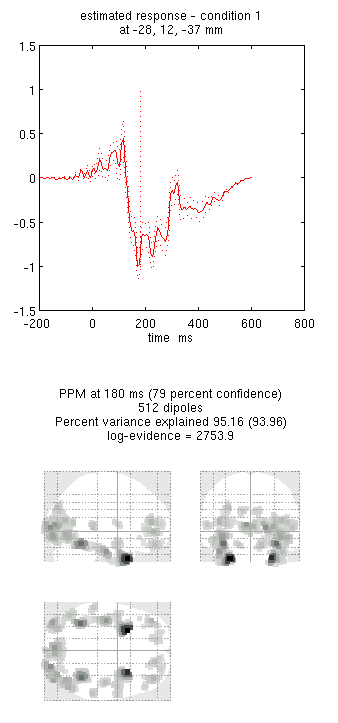
\includegraphics[width=90mm]{multimodal/figures/fused_eeg_meg_msp.png}
\caption{\em Graphical output of an MSP estimation of the differential evoked response between faces and scrambled faces at 170ms, after fusing both EEG and MEG data. \label{multimodal:fusion:fig:1}}
\end{center}
\end{figure}

To compare this ``fused'' inversion with individual inversion of the EEG or MEG data:

\begin{enumerate}
\item Press the ``new'' button and type ``N170'' as the label, press ``Invert'' again (note that all forward models are copied by default from the first inversion) and select the same options as above, except that when asked ``Multiple modalities'', press ``select'' this time, and select just ``EEG''. This should produce the results in Figure~\ref{multimodal:fusion:fig:2}.
\item Press the ``new'' button and type ``M170'' as the label, press ``Invert'' again and select the same options as above, except that when asked ``Multiple modalities'', press ``select'' and select just ``MEG'' this time. This should produce the results in Figure~\ref{multimodal:fusion:fig:3}.
\end{enumerate}

\begin{figure}
\begin{center}
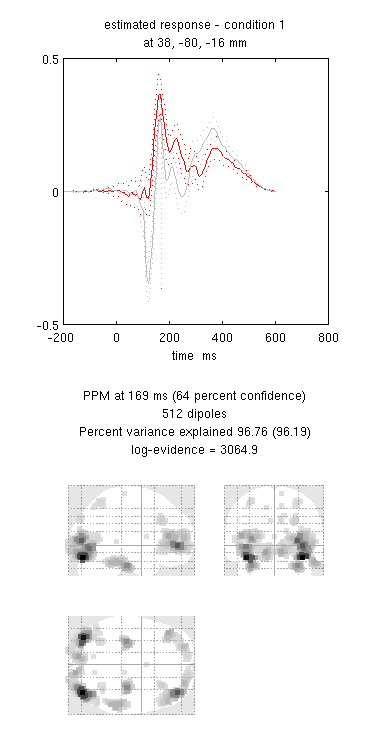
\includegraphics[width=90mm]{multimodal/figures/fused_eeg_msp.png}
\caption{\em Graphical output of an MSP estimation of the differential evoked response between faces and scrambled faces at 170ms, after inverting just EEG data. \label{multimodal:fusion:fig:2}}
\end{center}
\end{figure}

\begin{figure}
\begin{center}
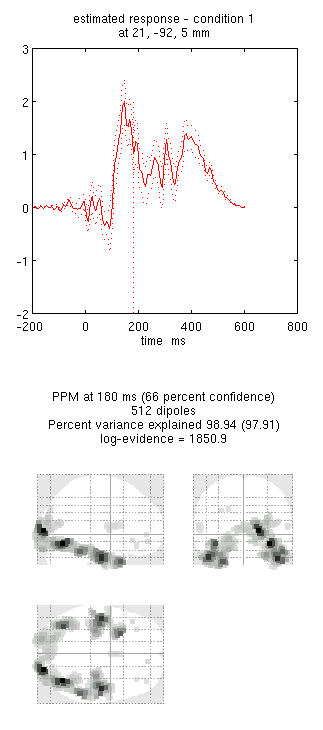
\includegraphics[width=90mm]{multimodal/figures/fused_meg_msp.png}
\caption{\em Graphical output of an MSP estimation of the differential evoked response between faces and scrambled faces at 170ms, after inverting just MEG data. \label{multimodal:fusion:fig:3}}
\end{center}
\end{figure}

By comparing these figures, you can see that the multimodal fused inversion (first inversion) combines aspects of both the unimodal inversions. Unfortunately one cannot simply compare the multi-modal vs uni-modal reconstructions via the log-evidence, because the data differs in each case (rather, one could use an estimate of the conditional precision of the sources, as in Henson et al, 2009b). With multiple subjects though, one could compare statistics across subjects using either multimodal or unimodal inversions.

\subsection{EEG, MEG and fMRI fusion \label{multimodal:fusion:fmri}}

Now we can examine the effects of using the fMRI data in Section~\ref{multimodal:data:fMRI} as spatial priors on the sources (Henson et al, in press).

First we need to create an 3D volumetric image of the clusters that we wish to use as spatial priors. These clusters can be defined by thresholding an SPM for a given fMRI contrast: here we will use the contrast in Section~\ref{multimodal:data:fMRI} of faces versus scrambled faces (using all three basis functions). So press ``Results'' and select the ``SPM.mat'' file from the ``fMRI/Stats'' directory. Select the previous faces vs scrambled F-contrast, do not mask or change title, use FWE correction at 0.05 and a 60-voxel extent to reproduce the SPM\{F\} shown in Figure~\ref{multimodal:fig:22} (if you are still in SPM's ``EEG'' mode, you will also be asked the type of images, for which you reply ``Volumetric 2D/3D'').

Now press the ``save'' button in the Interactive window and enter a filename like \texttt{Faces\-Vs\-Scrambled\_FWE05\_60}. This will produce a 3D image (which you can display as normal) in which all subthreshold voxels are set to zero (ie, where only 6 clusters containing non-zero voxel values are left).

Press ``fMRI priors'', and select the \texttt{uwmcdbespm8\_\-SPM\_\-CTF\_\-MEG\_\-example\_\-faces1\_\-3D.mat} file in the ``Fused'' directory. You will then be prompted for the image file that defines the thresholded clusters, for which you should select the \texttt{FacesVsScrambled\_\-FWE05\_\-60.img} file in the ``fMRI/Stats'' directory.
%%You will then be prompted for the grey matter (GM) image that was used to define the cortical mesh, for which you should select the ``c1smri.img'' file in the ``sMRI'' directory.
Finally, you will be asked whether the image is in Native or MNI space, which in this case is MNI space, because the fMRI images were spatially normalised.

A figure will appear, showing the location of each fMRI cluster as projected onto the cortical mesh.

A new image will be created (in the ``fMRI/Stats'' directory) called \texttt{cluster\_\-FacesVsScrambled\_\-FWE05\_\-60.img}, which contains the six binary priors, as will a new \matlab\ file called \texttt{priors\_\-uwmcdbespm8\_\-SPM\_\-CTF\_\-MEG\_\-example\_\-faces1\_\-3D\_\-1.mat}, which contains the information necessary to construct the covariance components for subsequent inversion.

Now press the ``new'' button to create a fourth inversion, and type ``N/M170+fMRI'' as the label.

To finish this with current state of code, press``save'', then 
\begin{verbatim}
	D  = spm_eeg_load('uwmcdbespm8_SPM_CTF_MEG_example_faces1_3D.mat');
	pQ = load('priors_uwmcdbespm8_SPM_CTF_MEG_example_faces1_3D_1.mat');
	D.val = 4;
	D.inv{4} = D.inv{1};
	D.inv{4}.inverse.pQ = pQ.pQ;
	D = spm_eeg_invert(D);
	D.save
	spm_eeg_invert_display(D);
\end{verbatim}

Then see Figure~\ref{multimodal:fusion:fig:4}.

%%press ``Invert'' again (note that all forward models are copied by default from the first inversion) and select the same options as above, except that when asked ``Multiple modalities'', press ``select'' this time, and select just ``EEG''. This should produce the results in Figure~\ref{multimodal:fusion:fig:5}.

\begin{figure}
\begin{center}
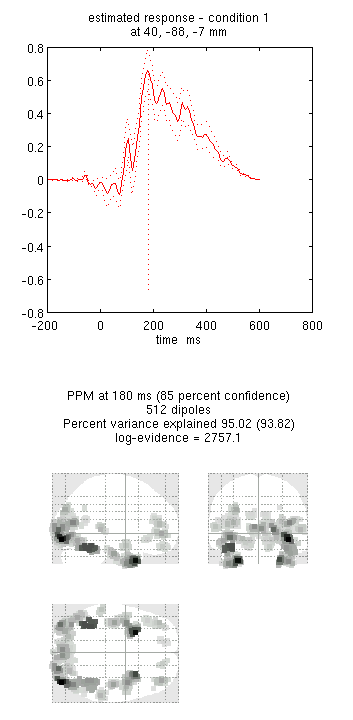
\includegraphics[width=90mm]{multimodal/figures/fused_eeg_meg_msp_fmri.png}
\caption{\em Graphical output of an MSP estimation of the differential evoked response between faces and scrambled faces at 170ms, after fusing EEG, MEG and fMRI data. \label{multimodal:fusion:fig:4}}
\end{center}
\end{figure}

You can repeat the above steps to use the common fMRI effect of faces and scrambled faces versus baseline (though at a higher threshold perhaps) as an alternative set of spatial priors for inverting either the differential evoked MEG/EEG response, or the mean evoked MEG/EEG response vs baseline.
